\documentclass[10pt,a4paper]{article}
\usepackage[margin=1in]{geometry}

\usepackage{mathtools}
\usepackage{array}
\usepackage[utf8]{inputenc}
\usepackage{amsmath}
\usepackage{amsthm}
\usepackage{amsfonts}
\usepackage[export]{adjustbox}
\usepackage{amssymb}
\usepackage{relsize}
\usepackage{color}
\usepackage{url}
\usepackage{esvect}
\usepackage{graphicx}
\usepackage{rotating}
\usepackage{cancel}
\usepackage{caption}
\usepackage{subcaption}
\usepackage{subfig}
\usepackage{listings}
\makeatletter
\newcounter{elimination@steps}
\newcolumntype{R}[1]{>{\raggedleft\arraybackslash$}p{#1}<{$}}
\def\elimination@num@rights{}
\def\elimination@num@variables{}
\def\elimination@col@width{}
\newenvironment{elimination}[4][0]
{
    \setcounter{elimination@steps}{0}
    \def\elimination@num@rights{#1}
    \def\elimination@num@variables{#2}
    \def\elimination@col@width{#3}
    \renewcommand{\arraystretch}{#4}
    \start@align\@ne\st@rredtrue\m@ne
}
{
    \endalign
    \ignorespacesafterend
}
\newcommand{\eliminationstep}[2]
{
    \ifnum\value{elimination@steps}>0\sim\quad\fi
    \left[
        \ifnum\elimination@num@rights>0
            \begin{array}
            {@{}*{\elimination@num@variables}{R{\elimination@col@width}}
            |@{}*{\elimination@num@rights}{R{\elimination@col@width}}}
        \else
            \begin{array}
            {@{}*{\elimination@num@variables}{R{\elimination@col@width}}}
        \fi
            #1
        \end{array}
    \right]
    & 
    \begin{array}{l}
        #2
    \end{array}
    &%                                    moved second & here
    \addtocounter{elimination@steps}{1}
}
\makeatother

\def\MapleInput#1{\noindent{{\small $>$ {\tt \color{MapleRed}{#1} }}}}
\def\MapleOutput#1{{\begin{center} \color{MapleBlue}{#1} \end{center}}}
\def\MapleWarning#1{\noindent{{\small {\tt \color{MaplePink}{#1} }}}}

\numberwithin{equation}{section}

\newcommand{\tvect}[3]{%
  \ensuremath{\Bigl(\negthinspace\begin{smallmatrix}#1\\#2\\#3\end{smallmatrix}\Bigr)}}


\usepackage[usenames,dvipsnames]{xcolor}
\definecolor{MapleRed}{rgb}{1,0,0}
\definecolor{MapleBlue}{rgb}{0,0,1}
\definecolor{MaplePink}{rgb}{1,0,1} 

\title{EMTH 211 Linear Algebra \\ Assignment}
\author{
  Danny Choo\\
  {\small student ID - 28842156}\\
  {\small kxc11@uclive.ac.nz}
  \and
  Grace Dain Lee\\
  {\small student ID - 51455525}\\
  {\small dil15@uclive.ac.nz}
}
\date{19th September 2016}




\begin{document}
	\maketitle
	\section*{Q1.a}
	\begin{figure}[h!]
		  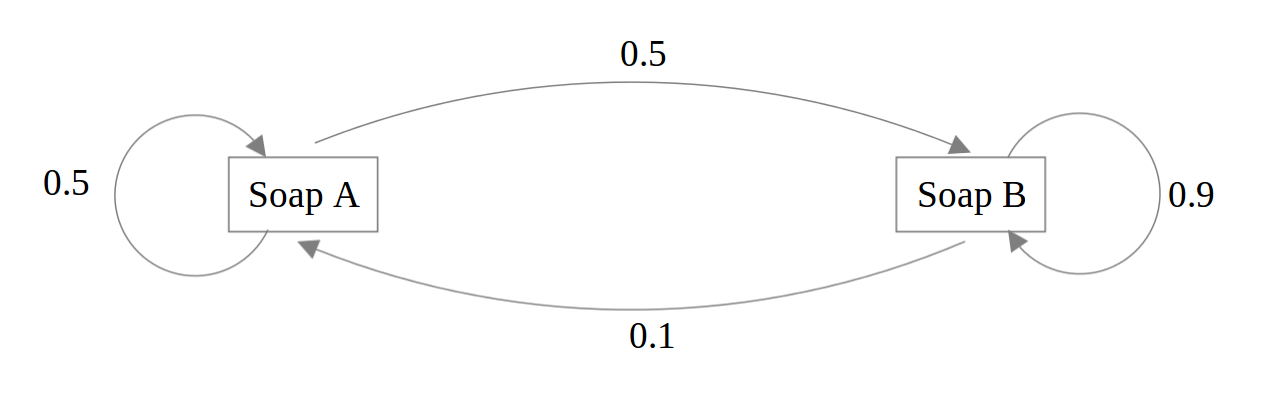
\includegraphics[width=\linewidth]{211_Image_edit.png}
		  \caption{A directed graph of the senario.}
		  \label{fig:boat1}
		\end{figure}
	
	
	
	Assume that, Soap A and B have 100 customers each at first\\
	\begin{align*}\label{eq1}
	A_{k}{\prime} = 0.5A_k + 0.1B_k \\	
	B_{k}{\prime} = 0.5A_k + 0.9B_k 	
	\end{align*}
	where $A_k$ = customers of soap A for this month and $B_k$ = customers of soap B for this month, and \\
	$A_{k}{\prime}$ = customers of soap A for next month and $B_{k}{\prime}$ = customers of soap B for next month. 
	\section*{Q1.b}
	\[\begin{bmatrix}
	A_{k}{\prime}\\
	B_{k}{\prime} 
	\end{bmatrix}
	=\begin{bmatrix}
	0.5 & 0.1 \\
	0.5 & 0.9
	\end{bmatrix}
	\begin{bmatrix}
	
	A_{k} \\
	B_{k}
	\end{bmatrix}\hfill\text{(from 1.1)}
	\]
	\\
	
	\noindent where  
	\[\begin{bmatrix}
		0.5 & 0.1 \\
		0.5 & 0.9
		\end{bmatrix}\]
		is the transition matrix.
		
	\section*{Q1.c}
	In one month's time
	
	
	\[\begin{aligned}\Rightarrow
	\begin{bmatrix}
		A_{k}{\prime}\\
		B_{k}{\prime} 
		\end{bmatrix}
		&=\begin{bmatrix}
		0.5 & 0.1 \\
		0.5 & 0.9
		\end{bmatrix}
		\begin{bmatrix}
		100 \\
		100
		\end{bmatrix}\\
		&=\begin{bmatrix}
		50 + 10 \\
		50 + 90
		\end{bmatrix}
		=\begin{bmatrix}
		60 \\
		140
		\end{bmatrix}\\	
		\end{aligned}
		\]
	\section*{Q1.d}
	In two month's time
		
		
		\[\begin{aligned}\Rightarrow
		\begin{bmatrix}
		A_{k}{\prime\prime}\\
		B_{k}{\prime\prime} 
		\end{bmatrix}
		&=\begin{bmatrix}
		0.5 & 0.1 \\
		0.5 & 0.9
		\end{bmatrix}
		\begin{bmatrix}
		A_{k}{\prime}\\
		B_{k}{\prime}
		\end{bmatrix}\\
		&=\begin{bmatrix}
		0.5 & 0.1 \\
		0.5 & 0.9
		\end{bmatrix}
		\begin{bmatrix}
		60 \\
		140
		\end{bmatrix}\\
		&=\begin{bmatrix}
		30 + 14 \\
		30 + 126
		\end{bmatrix}
		=\begin{bmatrix}
		44 \\
		156
		\end{bmatrix}\\	
		\end{aligned}
		\]
		where $A_{k}{\prime}{\prime}$ is the number of customers in two months time for soap A, and $B_{k}{\prime}{\prime}$ is the number of customers in two months time for soap B.
		
		\section*{Q1.e}
		In one year's time (12 months), the equation is:
		\[\begin{bmatrix}
		A_{k}{\prime\prime\prime}\\
		B_{k}{\prime\prime\prime} 
		\end{bmatrix}
		=\begin{bmatrix}
		0.5 & 0.1 \\
		0.5 & 0.9
		\end{bmatrix}^{12}
		\begin{bmatrix}
		100 \\
		100
		\end{bmatrix}
		\]
		\[\begin{aligned}
		\vv v_{1} = A^{12} \vv v_{0}.
		\end{aligned}\]
		\\
		This will be solved by finding eigenvectors and eigenvalues of the problem.\\
		
		\noindent To find the eignevalues:
		\begin{align*}
		det(A - \lambda I) = 0 \\
		det\begin{bmatrix}
		0.5 - \lambda & 0.1\\
		0.5 & 0.9 -\lambda\\		
		\end{bmatrix}=0\\
		\Rightarrow(0.5 -\lambda)(0.9 - \lambda) - 0.05 = 0\\
		\Rightarrow\lambda^2 - 1.4\lambda + 0.4 = 0\\	
		\Rightarrow 5\lambda^2 - 7\lambda + 2 = 0\\	
		\Rightarrow (5\lambda - 2)(\lambda - 1)= 0
		\end{align*}
		Hence, $\lambda_1$ = 0.4 and $\lambda_2$ = 1 \\
		
		\noindent To find the eigenvectors at $\lambda_1 = 0.4$,
		\\
		\[\begin{aligned}
		(A - \lambda_{1}I) \vv x_{1} = \vv 0
		\end{aligned}\]
		
		\begin{elimination}[2]{2}{1.1em}{1.1}% Decreased from 1.75em
		    \eliminationstep
		    {
		        0.1 & 0.1  & 0 \\
		        0.5 & 0.5  & 0 \\
		    }
		    {
		        \\
		        R_{2} -> R_{2}-5R_{1} \\
		    }
		    \eliminationstep
		    {
		        0.1 & 0.1 & 0  \\
		        0 &  0 &  0\\
		    }
		    {
		        \\
		        \\
		        \noindent 
		    }
		\end{elimination}
		So, $x_{1} = -x_{2}$.
		Thus, $\vv x_{1}$ =  
		$\begin{bmatrix}
		1 \\
		-1
		\end{bmatrix}$
		\\	
		\\	
			
		\noindent To find the eigenvectors At $\lambda_2 = 1$,
		
		\[\begin{aligned}
				(A - \lambda_{2}I) \vv x_{2} = \vv 0
				\end{aligned}\]				\begin{elimination}[2]{2}{1.65em}{1.1}% Decreased from 1.75em
	    \eliminationstep
	    {
	        -0.5 & \phantom{-}0.1  & 0 \\
	        \phantom{-}0.5 & -0.1  & 0 \\
	    }
	    {
	        \\
	     R_{2} -> R_{2}+R_{1} \\
		   }
	  \eliminationstep
		 {
	        -0.5 & \phantom{-}0.1 & 0  \\
	        0 & 0 &  0\\
		    }
		    {
		        \\
		        \\
	        \noindent
		    }
		\end{elimination}
		So, $x_{2} = 5x_{1}$.
		Thus, $x_{2}$ =  
		$\begin{bmatrix}
		1 \\
		5
		\end{bmatrix}$
		\\
		We know that $\vv v_{1} = A^{12}\vv v_{0}$, and $A = PDP^{-1}.$ Hence, finding $P, D, P^{-1}:$
		
	
		
		\[\ D=\begin{bmatrix}
				\lambda_{1} & 0 \\
				0 & \lambda_{2} 
				\end{bmatrix}
				=\begin{bmatrix}
				0.4 & 0 \\
				0 & 1
				\end{bmatrix}, 
				P = \begin{bmatrix}
					\phantom{-}1 & 1 \\
					-1 & 5
					\end{bmatrix},
				P^{-1} = \begin{bmatrix}
					\dfrac{5}{6} & -\dfrac{1}{6} \\[8pt]
					
					\dfrac{1}{6} & \phantom{-}\dfrac{1}{6}
					\end{bmatrix}
				\]
		\\
		So,
		\[\begin{aligned}
				\vv v_{1} = A^{12} \vv v_{0}
				\end{aligned}\]\\
		\[\begin{bmatrix}
		A_{k}{\prime\prime\prime}\\B_{k}{\prime\prime\prime}
		\end{bmatrix}
		=
		\begin{bmatrix}
		0.5 & 0.1\\ 0.5 & 0.9
		
		\end{bmatrix}^{12}
		\begin{bmatrix*}
		100 \\ 100
		\end{bmatrix*}\]\\
		Thus,
		\[\begin{aligned}\Rightarrow\vv{v}_1 = PD^{12}P^{-1} \vv{v}_0
				&=\begin{bmatrix}
						\phantom{-}1 & 1\\ -1 & 5
						\end{bmatrix}
						\begin{bmatrix}
						0.4^{12} & 0\\ 0 & 1^{12}
						\end{bmatrix}
						\begin{bmatrix}
						\dfrac{5}{6} & -\dfrac{1}{6} \\[8pt]
						\dfrac{1}{6} & \phantom{-}\dfrac{1}{6}
					\end{bmatrix}\begin{bmatrix}
					100 \\ 100
					\end{bmatrix}					
				\end{aligned}
				\]\\
				
				\noindent The calculation was implemted via matlab.
				Matlab shows
				\lstinputlisting[language=Matlab]{Q1.e.txt}
				which is correct.
				\\
				
				\noindent In the long run:\\
			
				\begin{align*}
				\vv v_{k} & = A^k\vv v_{0}\\&= PD^{k}P^{-1} \vv{v}_0\\&=\begin{bmatrix}
				\phantom{-}1 & 1 \\ -1 & 5
				\end{bmatrix}
				\begin{bmatrix}
				\phantom{-}0.4^k & 0 \\ 0 & 1^k
				\end{bmatrix}	
				\begin{bmatrix}
				\dfrac{5}{6} & -\dfrac{1}{6} \\[6pt]
				\dfrac{1}{6} & -\dfrac{1}{6}
				\end{bmatrix}
				\begin{bmatrix}
				100 \\ 100
				\end{bmatrix}
				\end{align*}
			\\
			
			\noindent As $k \rightarrow \infty$,
			\begin{align*}
			D^\infty = \begin{bmatrix} 0 & 0 \\ 0 & 1
			\end{bmatrix}
			\end{align*}
			
			\begin{align*}
							\vv v_{k} &=\begin{bmatrix}
							1 & 1 \\ -1 & 5
							\end{bmatrix}
							\begin{bmatrix}
							0 & 0 \\ 0& 1
							\end{bmatrix}	
							\begin{bmatrix}
							\dfrac{5}{6} & -\dfrac{1}{6} \\[6pt]
							\dfrac{1}{6} & -\dfrac{1}{6}
							\end{bmatrix}
							\begin{bmatrix}
							100 \\ 100
							\end{bmatrix}\\
							&=\begin{bmatrix}
							0 & 1 \\ 0 & 5
							\end{bmatrix}	
							\begin{bmatrix}
							\dfrac{5}{6} & -\dfrac{1}{6} \\[6pt]
							\dfrac{1}{6} & -\dfrac{1}{6}
							\end{bmatrix}
							\begin{bmatrix}
							100 \\ 100
							\end{bmatrix}\\
							&=	
							\begin{bmatrix}
							\dfrac{1}{6} & \dfrac{1}{6} \\[6pt]
							\dfrac{5}{6} & \dfrac{5}{6}
							\end{bmatrix}
							\begin{bmatrix}
							100 \\ 100
							\end{bmatrix}\\[0.5em] & = \begin{bmatrix}
							\dfrac{200}{6} \\[1em] \dfrac{1000}{6} \\
							\end{bmatrix}
							\end{align*}
			Since, \begin{align*}
			\Rightarrow \dfrac{200}{6} + \dfrac{1000}{6} =\dfrac{1200}{6} = 200
			\end{align*}
			The solution is correct.
					 
	\section*{Q1.f}
		
		As worked out in Q1e, $Ax$ = $\lambda x$, then
		\begin{align*}
		\Rightarrow Ax - \lambda x\\
		\Rightarrow (A - \lambda I) = 0\\	
		\end{align*}
		when $\lambda$ = 1, \\
				
		\begin{elimination}[2]{2}{1.65em}{1.1}% Decreased from 1.75em
	   \eliminationstep
	    {
		    -0.5 & \phantom{-}0.1  & 0 \\
		    \phantom{-}0.5 & -0.1  & 0 \\
		    		    }
	    {
			     \\
	    R_{2} -> R_{2}+R_{1} \\
		    }
	    \eliminationstep
		    {
	        -0.5 & 0.1 & 0  \\
	        0 &  0 &  0\\
	    }
	    {
	        \\
	        \\
	        x_{1} = -x_{2}
	    }
	\end{elimination}
	As done in Q 1.e, the eigenvector of $\lambda$ = 1 is $x$ =  
		$\begin{bmatrix}
			1 \\
			5
		\end{bmatrix}.$
		
		
	\section*{Q2.a}
	\subsubsection*{(i)}
	\lstset
	{ %Formatting for code in appendix
	    language=Matlab,
	    basicstyle=\footnotesize,
	    numbers=left,
	    stepnumber=1,
	    showstringspaces=false,
	    tabsize=1,
	    breaklines=true,
	    breakatwhitespace=false,
	}
	The function is written as below

	\lstinputlisting[language=Matlab]{power_method.m}
	
	\noindent The approximated eigenvalue and the corresponding eigenvalue was tested with the test file below:
	\lstinputlisting[language=Matlab]{test2.m}
	
	\noindent After running the above program, the output is shown as:
	
	\lstinputlisting{minion.txt}
	
	\noindent as expected.
	
	
	\newcommand{\fourones}{\begin{bmatrix}
					1 \\
					1\\
					1\\
					1
			\end{bmatrix}}
			
	\newcommand{\Ay}{\begin{bmatrix}
					-2.7\\
					6.9\\
					2\\
					-9.6 
					\end{bmatrix}}
					
	\newcommand{\Ayone}{\begin{bmatrix}
								-0.28128\\
								0.71375\\
								0.20833\\
								-1
						\end{bmatrix}}
						
	\newcommand{\A}{\begin{bmatrix}
			-3.9 & 0.1 & 0.5 & 0.6\\
			0.1 & 7.2 & 0.1 & -0.5\\
			0.5 & 0.1 & 1.1 & 0.3\\
			0.6 & -0.5 & 0.3 & -10 
			\end{bmatrix}}
			
	\subsubsection*{(ii)}
	
	\lstset
		{ %Formatting for code in appendix
		    language=Matlab,
		    basicstyle=\footnotesize,
		    numbers=left,
		    stepnumber=1,
		    showstringspaces=false,
		    tabsize=1,
		    breaklines=true,
		    breakatwhitespace=false,
		}
		Similarly, the Inverse power method function is written as below
	
		\lstinputlisting[language=Matlab]{inverse_method.m}
		
		\noindent The approximated eigenvalue and the corresponding eigenvalue was tested with the test file below:
		\lstinputlisting[language=Matlab]{test.m}
		
		\noindent After running the above program, the output is shown as:
		
		\lstinputlisting{minion2.txt}
		
		\noindent as expected.
	
	
	
	
	\section*{Q2.b}
	\subsubsection*{(i)}

		\[\begin{aligned}A =
			\begin{bmatrix}
				-3.9 & 0.1 & \phantom{-}0.5 & \phantom{-}0.6\\
				\phantom{-}0.1 &\phantom{-}7.2 & \phantom{-}0.1 & -0.5\\
				\phantom{-}0.5 & \phantom{-}0.1 & \phantom{-}1.1 & \phantom{-}0.3\\
				\phantom{-}0.6 & -0.5 & \phantom{-}0.3 & -10 
				\end{bmatrix}
				\end{aligned}
				\]\\
				Using the power method function in Q2a, the dominant eigenvalue is -10.0782, and the corresponding eigenvector is
				\[\begin{bmatrix}
					0.0953 \\ -0.0222\\0.0228\\-0.9949
					\end{bmatrix}\]

	\subsubsection*{(ii)}
	The Gerschgorin Disks Diagram is attached on a separate page.\\
	Using the inverse power method matlab function written in Q2a, the approximations were found to be \lstinputlisting{minion2.txt}
	
	
		
	
	
	
		
	\section*{Q3}
	\subsubsection*{(a-d)}
	See attached.
	
	\subsubsection*{(e)}
	The higher degree fits become less reliable than ones of lower degree because the least squares method works best for data that is relatively linear. As the polynomial order increases, it deviates further from the original function. Hence, the least squares method is not effective for higher degree polynomials.
	
	
	\newpage
	
	\begin{figure}[h!]
	  \begin{sideways}
	  
	      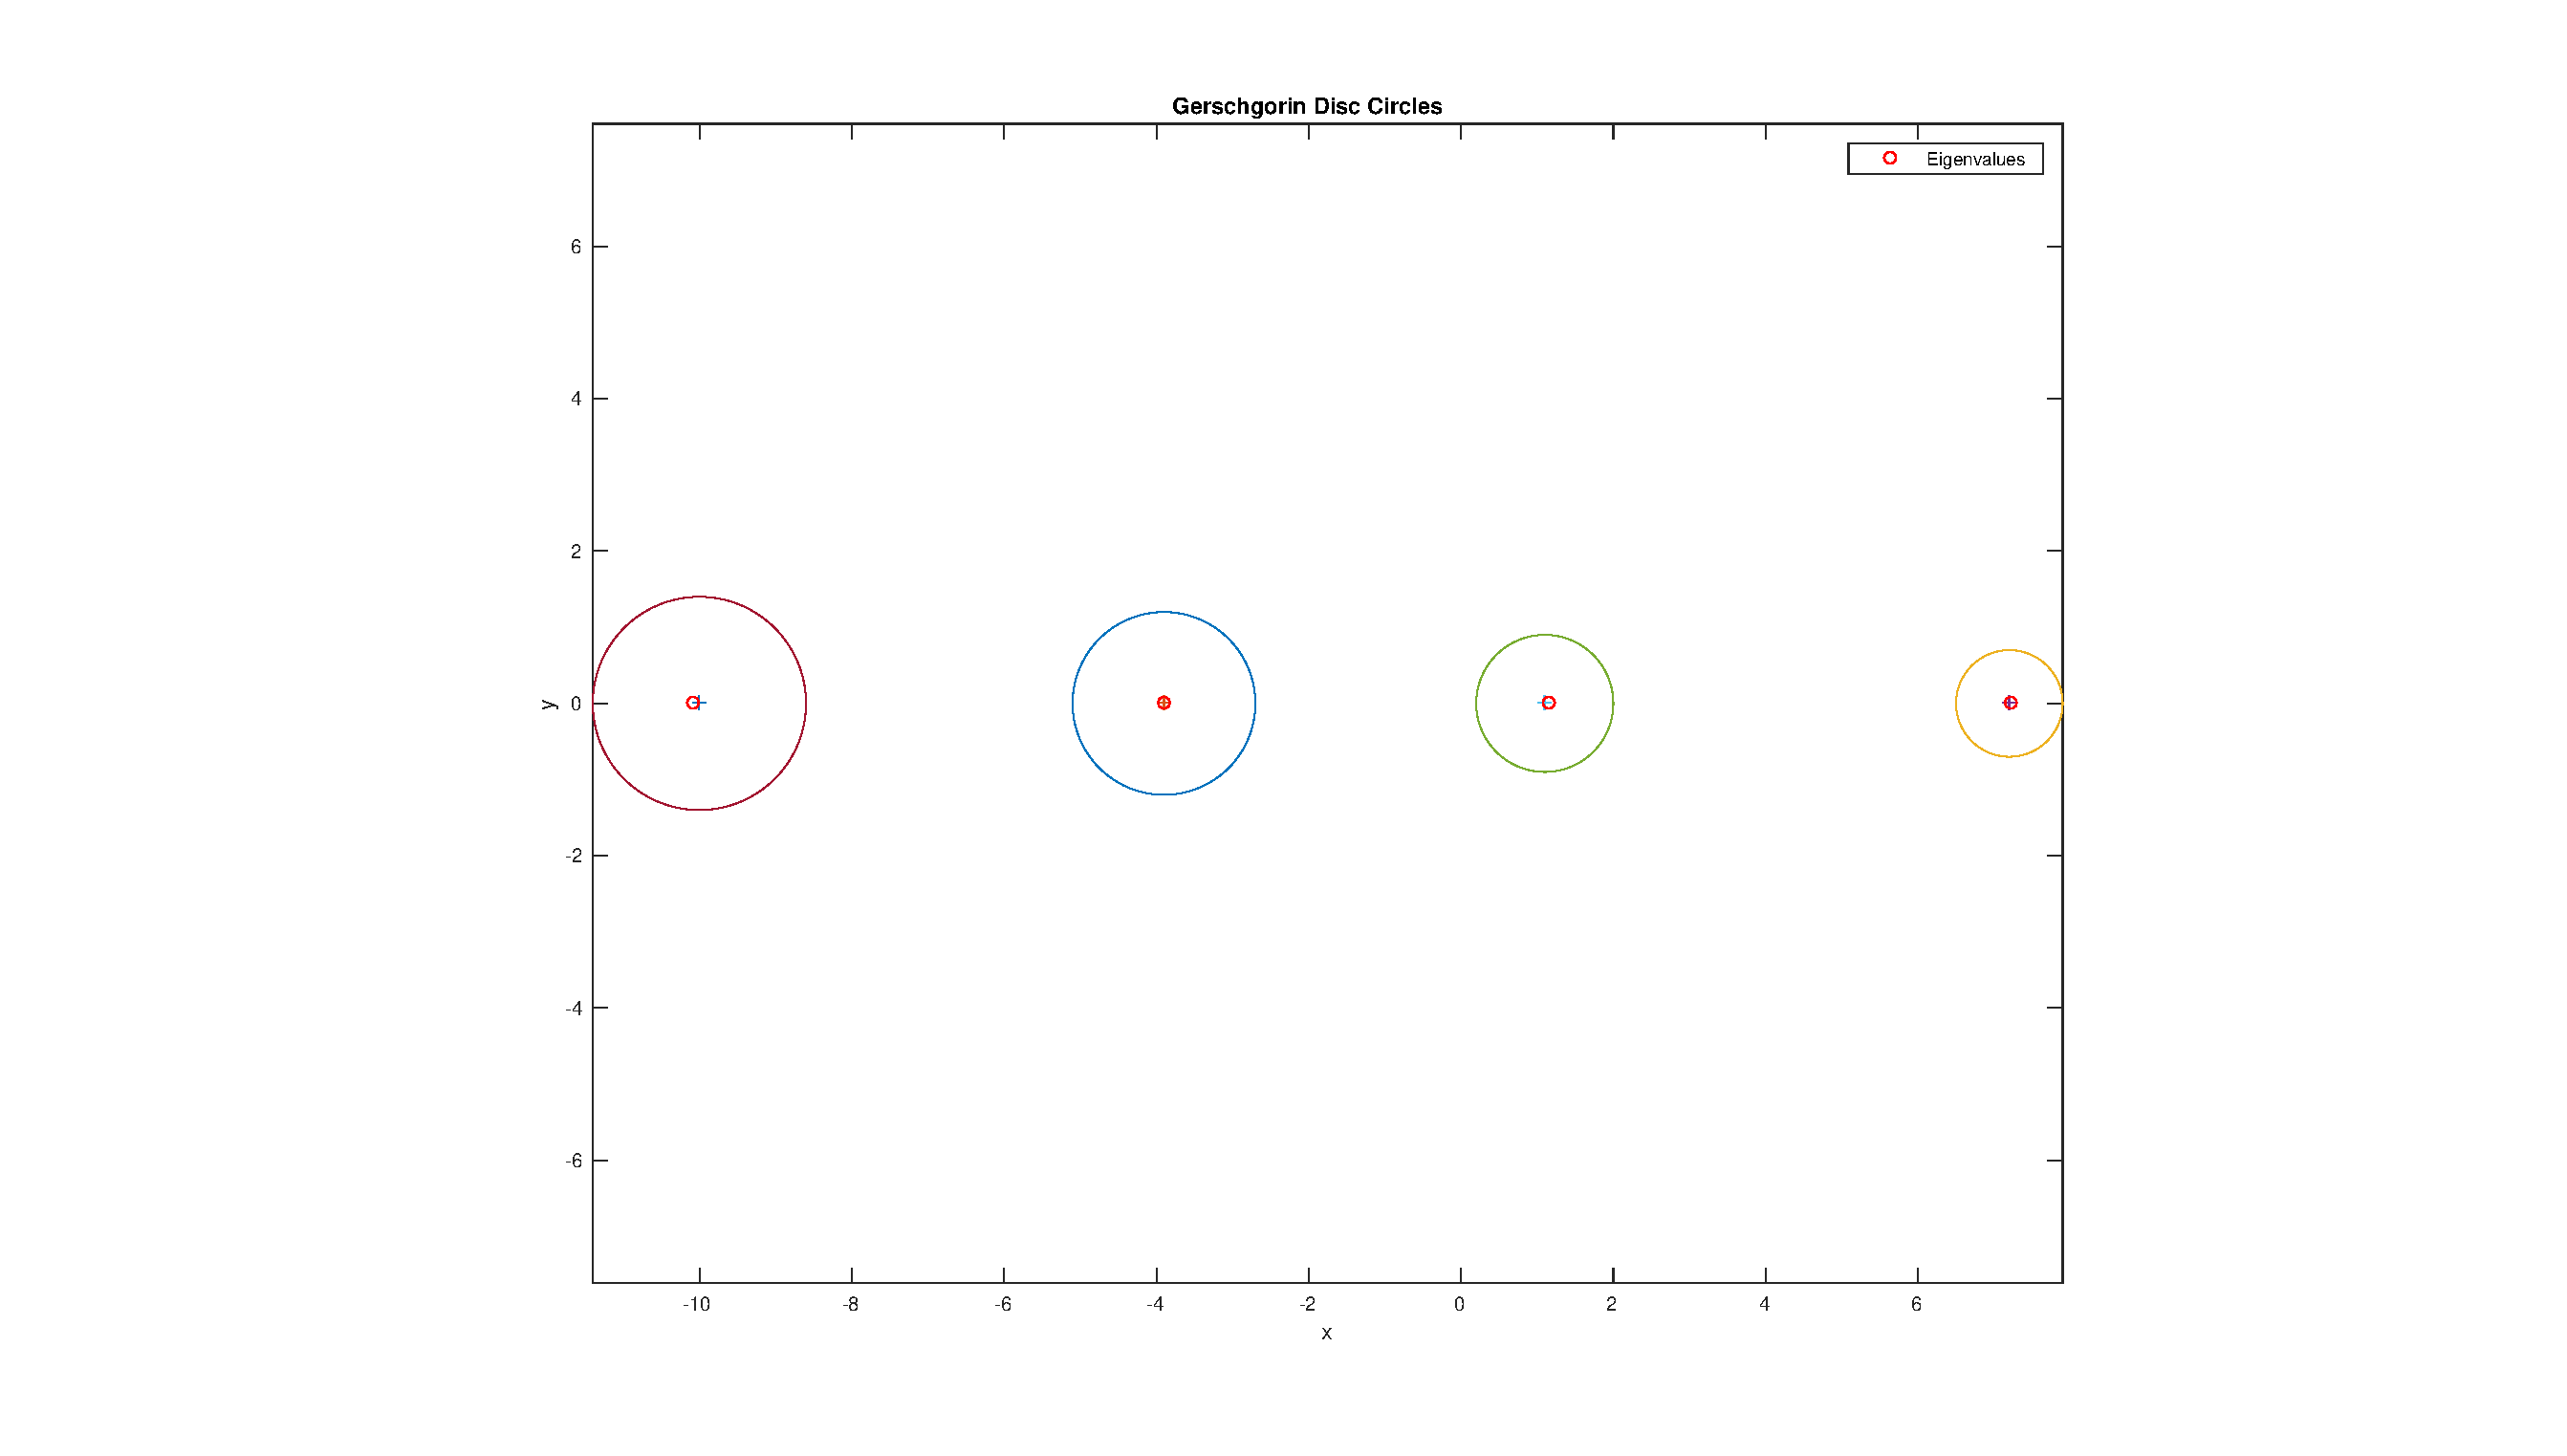
\includegraphics[width=2\textwidth,center]{gersch.eps}
		  \end{sideways}
	  \centering
	  \label{pic:picture}
	\end{figure}
	
	\newpage
			
	\begin{figure}[hb!]
	\begin{sideways}
	\centering
				  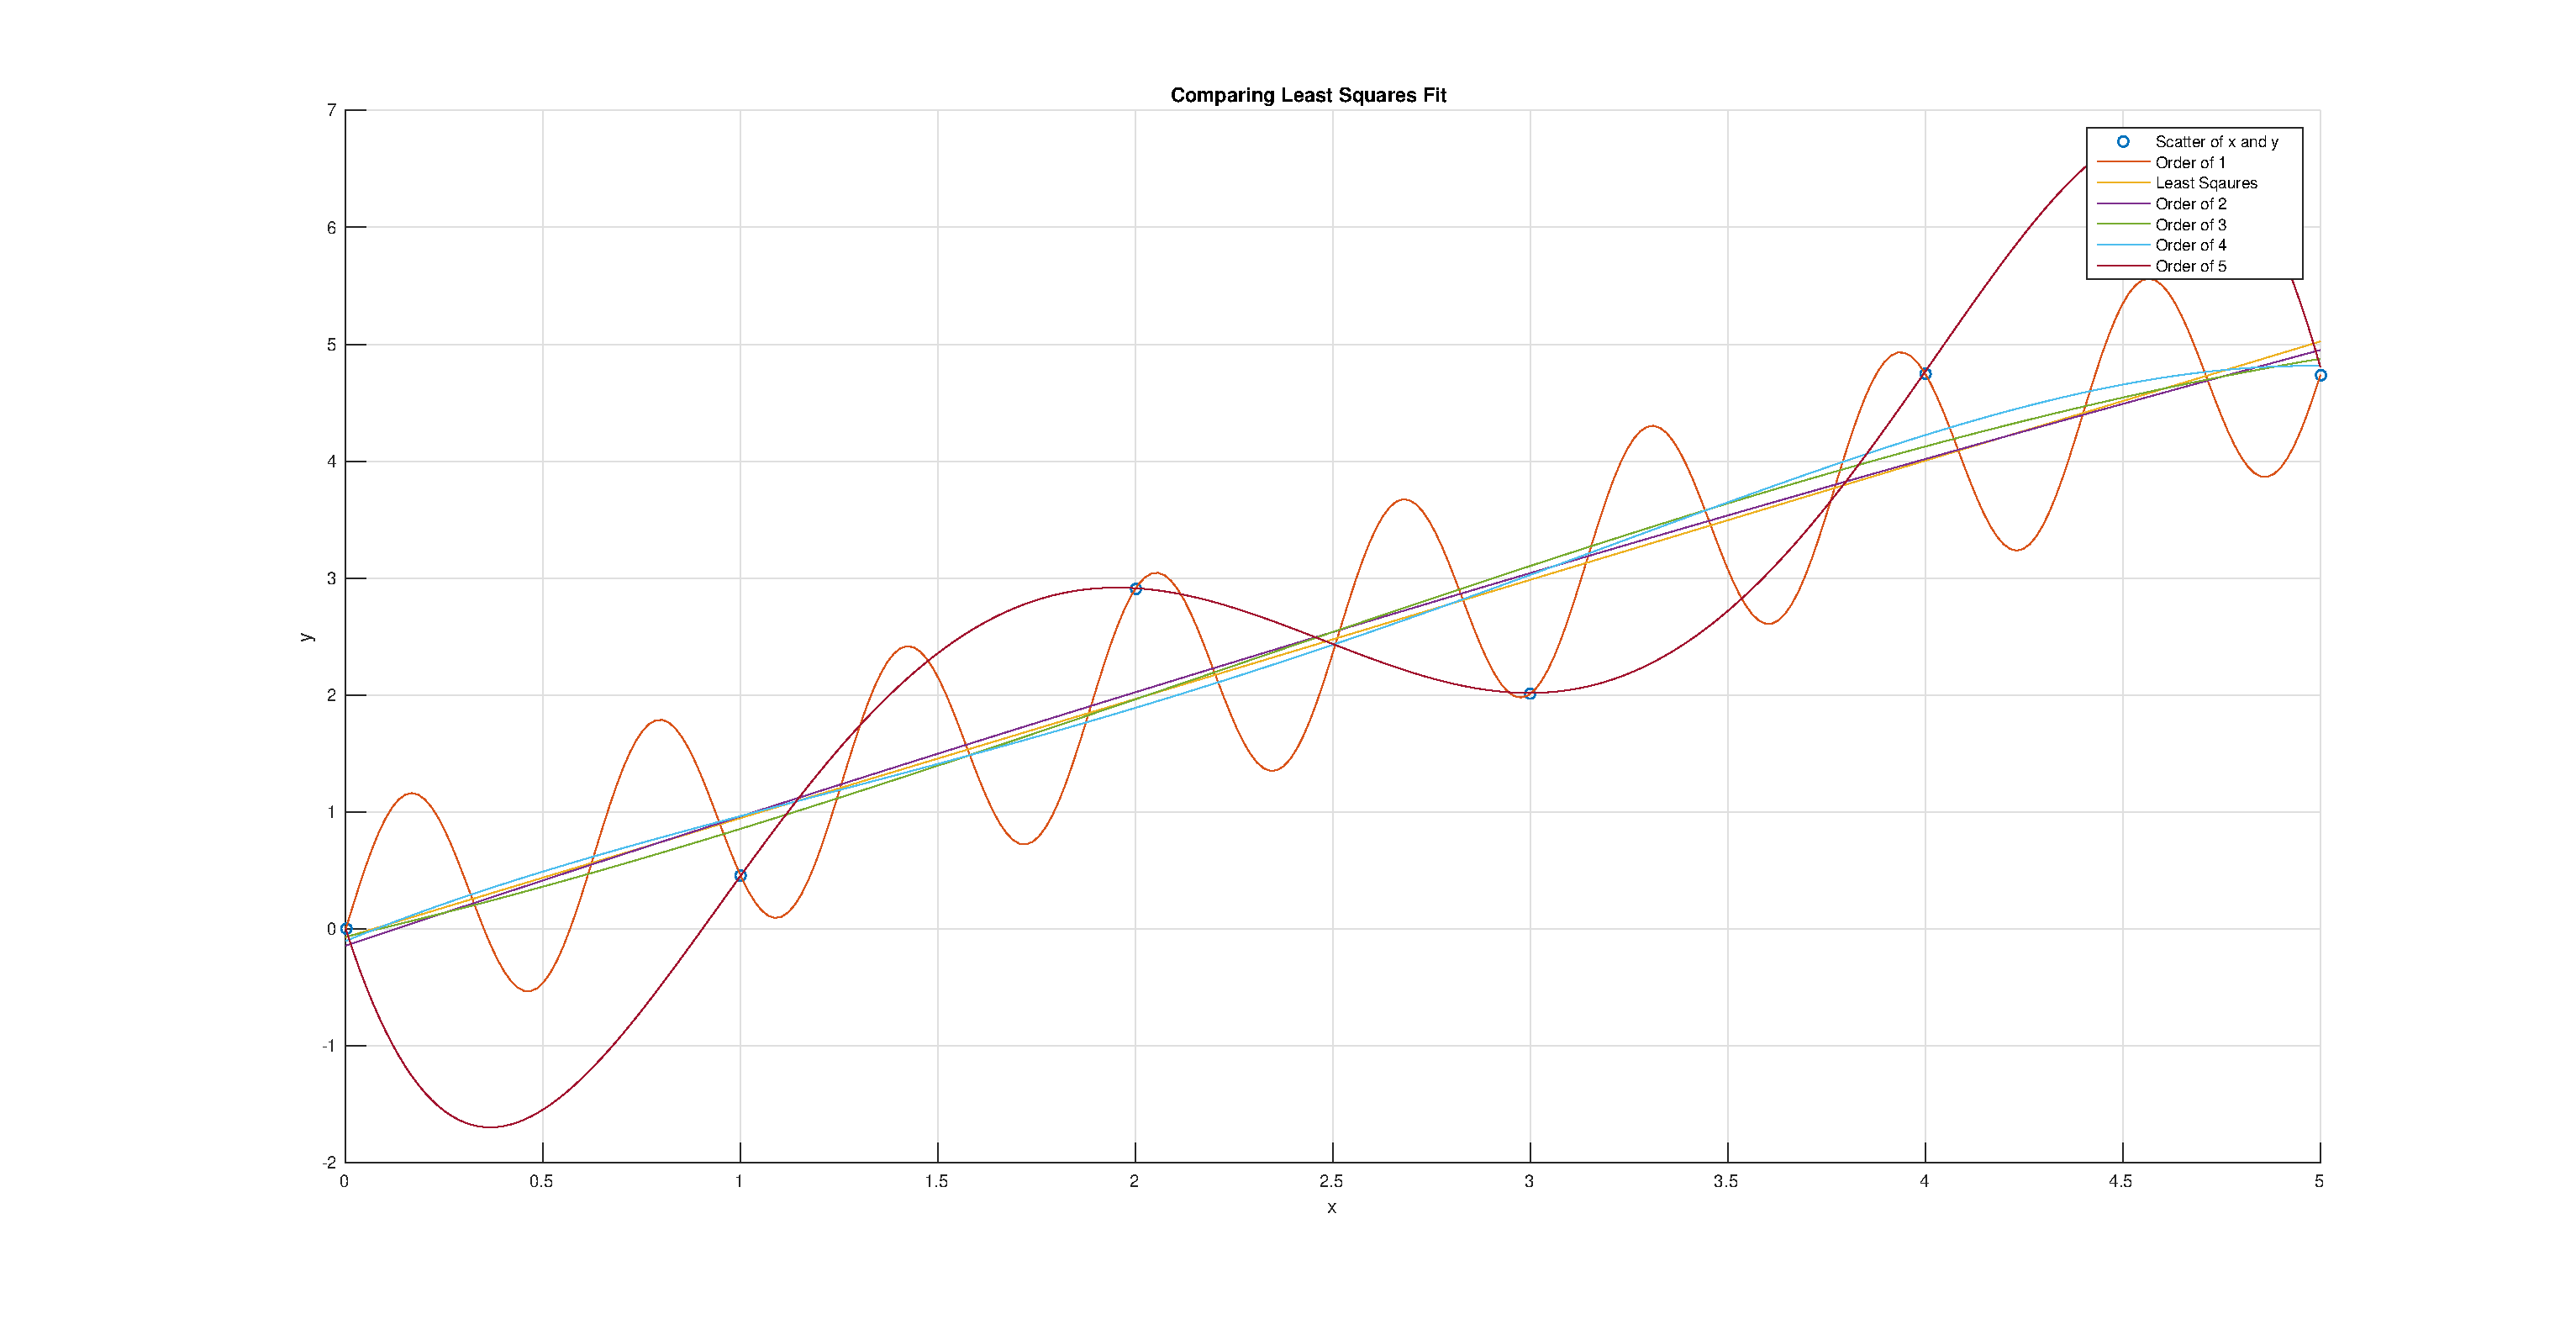
\includegraphics[width=1.8\textwidth,right]{Q3_graphs.eps}
				
				  \end{sideways}
				  \label{fig:boat1}
				\end{figure}
	

\end{document}
